% !TeX spellcheck = cs_CZ
\begin{mdframed}[style=mdexam]
  \begin{example}
    Stanovte intenzitu magnetického pole $H=f(r)$ dlouhého dutého válcového vodiče podle obr.
    \ref{TEMP:fig_pole_duty_valec} při rovnoměrném rozložení proudu $I$ po průřezu. 
    
    {\centering
      \captionsetup{type=figure}
      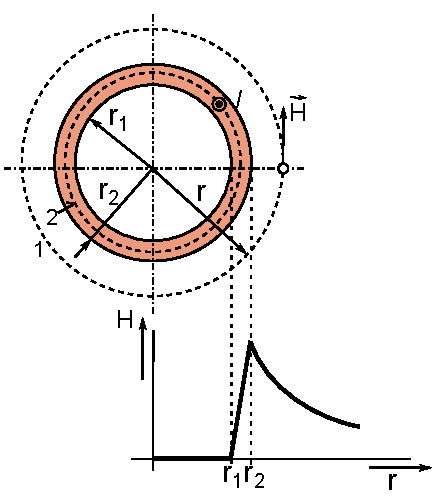
\includegraphics[width=0.5\linewidth]{duf_duty_valec_H.pdf}
      \captionof{figure}{K příkladu stanovení intenzity magnetického pole dlouhého dutého válcového 
                vodiče protékaného proudem}
      \label{TEMP:fig_pole_duty_valec}
    \par}
    
    Vodič s rovnoměrně rozloženým proudem podle obr. \ref{TEMP:fig_pole_duty_valec} je rotačně
    souměrný podle své osy a tedy i jeho magnetické pole je souměrné. Silové čáry jsou soustředné
    kružnice, vektor $\vr{H}$, jenž má směr tečny ke kružnici, je po celé délce kružnice stejně
    velký. Lze tedy snadno použít integrálního tvaru 1. MR (\textbf{zákon celkového proudu})
    
    Pro body ležící vně vodiče obepíná kruhová integrační dráha (vedená po silové čáře 1) celý
    proud vodiče $I$ a platí
    \begin{equation}\label{TEMP:eq_1MR_duty_valec}
      \oint_{\mathcal{C}}\vr{H}d\vr{l} = H\cdot 2\pi r = I
    \end{equation}
    takže intenzita pole je
    \begin{equation}\label{TEMP:eq_H_duty_valec}
      H = \frac{I}{2\pi r}
    \end{equation}
    
    Ve stěně dutého magnetického vodiče jsou silové čáry rovněž kružnice, neboť magnetické pole
    je i zde souměrné. Tyto siločáry však obepínají jen část proudu $I'$ vodiče pro oběh siločáry
    2 platí
    \begin{equation}\label{TEMP:eq_1MR_uvnitr_valce}
      \oint_{\mathcal{C}}\vr{H}d\vr{l} = H\cdot 2\pi r = I' = \pi(r^2-r_1^2)J
    \end{equation}
    kde $J$ je hustota proudu ve vodiči
    \begin{equation}\label{TEMP:eq_J_duty_valec}
      J = \frac{I}{S}= \frac{I}{\pi(r_2^2-r_1^2)}
    \end{equation}
    Ve stěně vodiče je tedy intenzita pole
    \begin{equation}\label{TEMP:eq_H_uvnitr_valce}
      H = \frac{I}{2\pi r}\frac{r^2-r_1^2}{r_2^2-r_1^2}
    \end{equation}
    V dutině vodiče je intenzita rovna nule. Vzhledem k souměrnosti pole by i zde muselo platit
    $\oint_{\mathcal{C}}\vr{H}d\vr{l} = H\cdot 2\pi r$. Protože dráha s poloměrem $r<r_1$ neobepíná
    žádný proud, je $\oint_{\mathcal{C}}\vr{H}d\vr{l} = 0$ a tedy musí byt $H = 0$.
  \end{example}    
\end{mdframed}